\subsection{Network Entity}
Every object that is going to send/receive data is going to do so via a \emph{Network Entity}.
A \emph{Network Entity} consists of three parts.
\begin{itemize}
\item NetworkEntityShared
\item NetworkEntityServer
\item NetworkEntityClient
\end{itemize}

The \emph{NetworkEntityShared} holds all the information both needed by the server and the client, about the object.
Information like the position and rotation are stored for basic synchronization.

Each \emph{NetworkEntityShared} has a unique id, which is the same on all connected players.
That is, if an enemy is spawned on the server, the server will give the enemy an id, and then send instructions to the client to create an enemy at the same position, with the same id.

\emph{NetworkEntityServer} inherits \emph{NetworkEntityShared} and extends with a method to send the position and rotation of the object to which it is attached, as well as a method to receive input if it is a player controlled object.

\emph{NetworkEntityClient} also inherits from \emph{NetworkEntityShared} and extends with a method to receive a position and rotation of the object in order to correct it, as well as a method to send input if it is a player controlled object.

When an object that needs to be synchronized is spawned, on the server it gets a \emph{NetworkEntityServer} and on the client a \emph{NetworkEntityClient}.
On both computers the network entities are given the same id, such that communication can be filtered so data does not get sent to or received by the wrong network entities.
This is illustrated on Figure \ref{fig:networkEntity}.

\begin{figure}
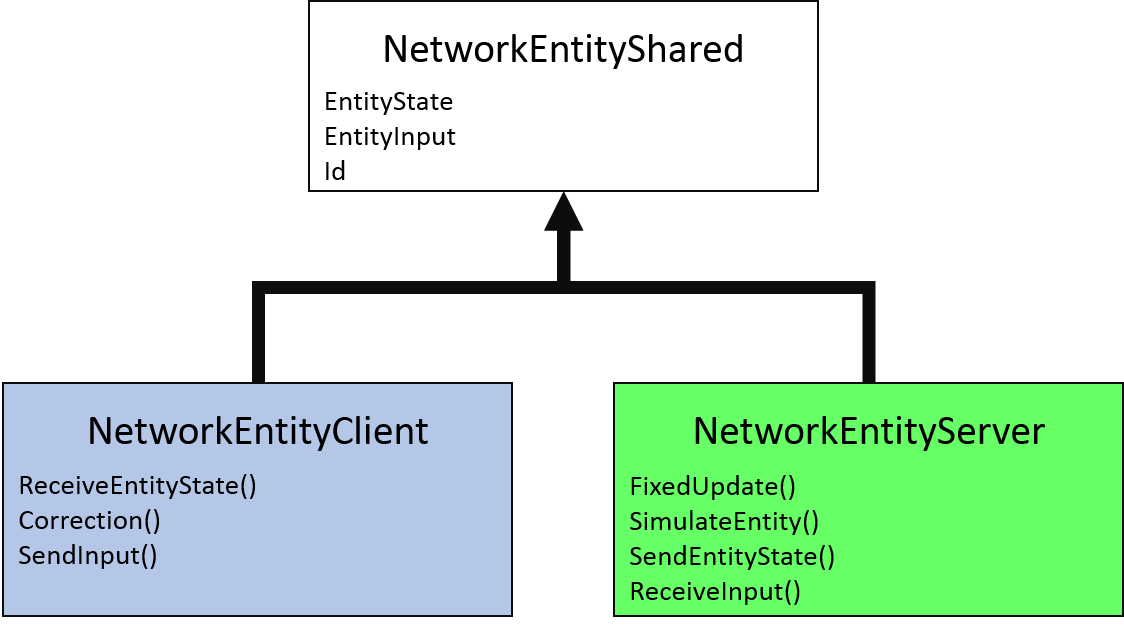
\includegraphics[scale=0.5]{figures/network/networkEntity}
\caption{An illustration of the connections between \emph{NetworkEntityClient} and \emph{NetworkEntityServer}.}
\label{fig:networkEntity}
\end{figure}

\subsection{NetworkHandler}
When the network entities need to synchronize and send/receive data, they do so through the \emph{NetworkHandler}.
This means that the \emph{NetworkHandler} handles all networking traffic.
The reason for this is that the \emph{NetworkHandler} then filters all the sent data by the id, such that each network entity only receives the data sent by its counterpart on the other device.
This also allows for network entities to not have to worry about who to send that data to or who it is receiving data from, only what data to send and receive.
Figure \ref{fig:networkHandler} illustrates how the \emph{NetworkHandler} filters data between a network entity being synchronized.

\begin{figure}
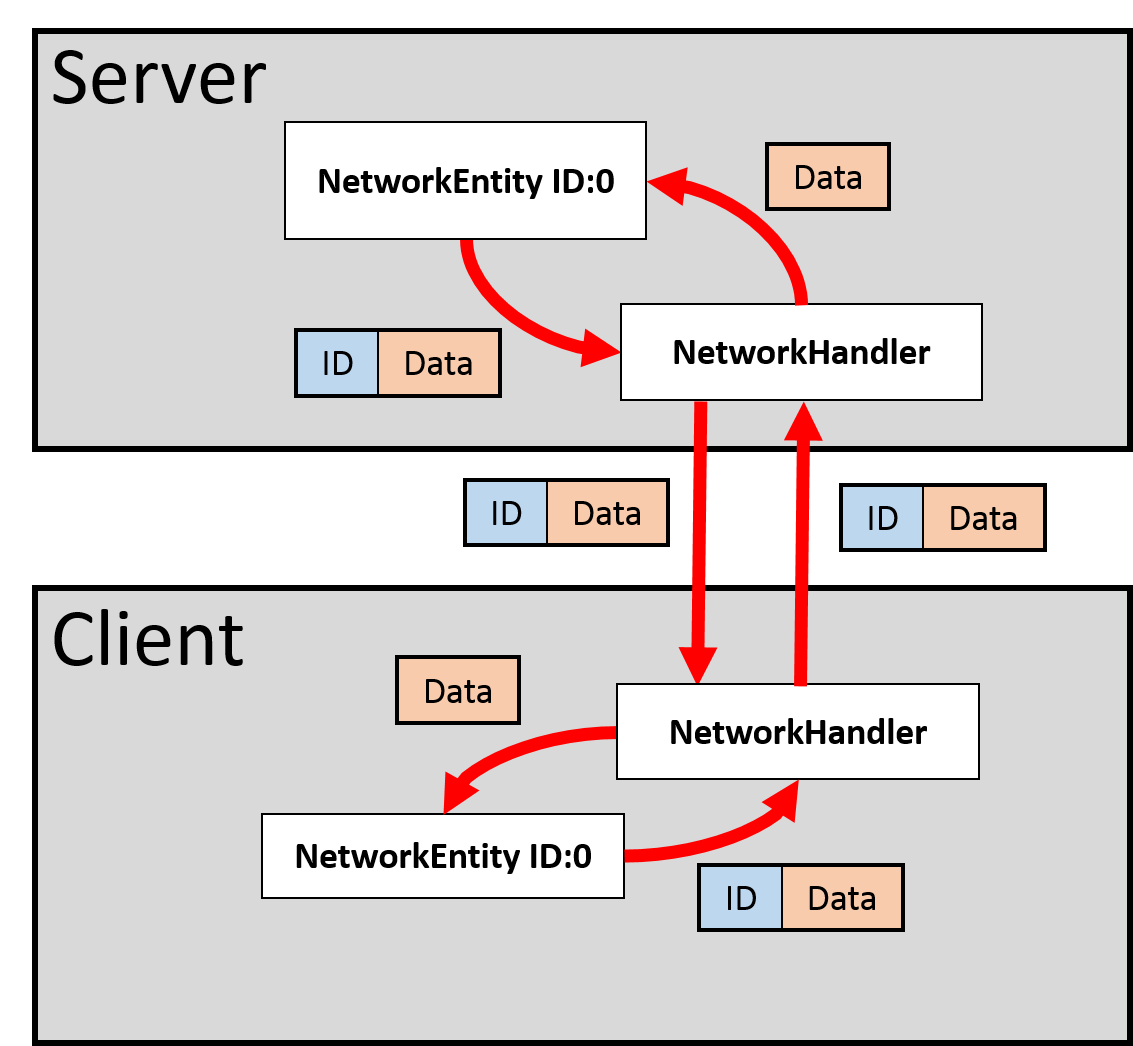
\includegraphics[scale=0.5]{figures/network/networkHandler}
\caption{An overview of how the \emph{NetworkHandler} uses the id to filter data from a unique entity to its own counterpart on another device.}
\label{fig:networkHandler}
\end{figure}